%%
%% Time-stamp: <2022-01-25 15:58:45 stefan>
%%
%% En CV i ett två-kolumn format
%%
%% Inspirerad av Kevin Fox (@fury.com) CV
%%

\documentclass[a4paper,swedish,10pt]{article}

\usepackage[utf8]{inputenc}

% fet för rubriker
\usepackage{tgadventor}

% brödtext
\usepackage[scaled=1.0]{gillius2}
\renewcommand*{\familydefault}{\sfdefault}

% specialfont för årtal
\usepackage{cinzel}
\usepackage[T1]{fontenc}    %% annars fungerar inte klipp-och-klistra från PDF självt

\usepackage{calc}
\usepackage{babel}
\usepackage[a4paper,top=2cm,bottom=2cm,left=1.5cm,right=1.5cm]{geometry}
\usepackage{fullminipage}
\usepackage{xcolor}
\usepackage{graphicx}
\usepackage[export]{adjustbox}
%% \usepackage{ragged2e}
\usepackage{enumitem}
\usepackage{blindtext}
\usepackage{adjustbox}
\usepackage[colorlinks=true, allcolors=blue]{hyperref}

\usepackage{fancyhdr}
\setlength{\headheight}{35pt}
%\addtolength{\topmargin}{-22pt}
\fancyhf[LH]{Stefan Skoglund\\Högalidsgatan 36\\521 61 Stenstorp}
\fancyhf[CH]{%
  stefan.skoglund@agj.net\\%
  \href{http://www.linkedin.com/in/stefan-niskanen-skoglund-902aa0a1}{Linkedin:Stefan Skoglund}\\
  \href{https://github.com/Skaraborgfakir}{github: Skaraborgfakir}}
\fancyhf[RH]{%
  0500--450 878\\0702--719 835
}
\fancyhf[CF]{\href{https://skaraborgfakir.github.io/cv_minipage_2022.pdf}{Länk till aktuell version}}
\pagestyle{fancy}

\newenvironment*{descriptioncv}[1]%
{%
  \textbf{\large #1}%
  \begin{description}[nosep,font=\sffamily\bfseries, leftmargin=0.5cm, style=nextline]%
  }%
  {\end{description}\vspace{0.4cm}}
\newcommand*{\cvitem}[3]{\item[#1]{\cinzel#2}\\#3}

% DEBUG:utmatning av uppgifter om storlekar,kerning osv
\showoutput
\begin{document}

\begin{minipage}[t]{0.73\textwidth}
  \begin{descriptioncv}{Utbildningar och separata kurser}
    \cvitem{Lexicon, Göteborgs}{December 2021}{AZ900:certifiering}
    \cvitem{Lexicon, Göteborgs}{Juni 2021-December 2021}{Utbildning i dotNet:programmering med JavaScript,C\#, HTML, CSS, Azure och Entity Framework med dess Identity server}
    \cvitem{Lexicon, Göteborgs}{Mars 2021}{Gått igenom Lexicons Test\&Bedömning för deras support- och dotNET-utbildningar}
    \cvitem{Historia A, Göteborgs universitet}{Januari-- Juni 2018}{A:grundkursen i historia}
    \cvitem{Historia B, Göteborgs universitet}{Augusti-- December 2018}{Fortsättningskurs i historia, I B:uppsatsen använder jag  en Umeåprästs livshistoria som en källa}
    \cvitem{Skriptprogrammering i Linux, Göteborgs universitet}{Våren 2019}{telemetri med \texttt{awk} och \texttt{bash}, del av ett mätteknikprogram vid Chalmers}
    \cvitem{YH:utbildning, Signaltekniker, Lärcenter i Falköping}{Augusti 2014--Juni 2015}{inriktning mot ERTMS, växlar, spårledningar vägskydd, ställverk 59 och kommunikation mellan EBISAT och DLC }
    \cvitem{Databasteknik A, Högskolan i Skövde}{2019}{grundläggande databaskonstruktion i MySQL}
    \cvitem{Datornätverk A, Högskolan i Skövde}{2019}{CISCO ICND1}
    \cvitem{Linux administration A, Högskolan i Skövde}{2014}{UNIX admin: epost med web:gränssnitt}
    \cvitem{UNIX B, Högskolan i Skövde}{2012}{UNIX admin: epost med web:gränssnitt}
    \cvitem{C:programmering, Högskolan i Skövde}{1993}{programmeringsspråket C}
    \cvitem{Modellering, Högskolan i Skövde}{2018}{UML med grupporienterad verksamhetsmodellering}
  \end{descriptioncv}
  \begin{descriptioncv}{Arbeten}
    \cvitem{Signaltekniker, NVBS}{2017 Maj-- Augusti}{Uthyrd för ny- och ombyggnads-arbeten i samband
      med att Citybanan i Stockholm skulle öppnas. Förberedelser för Getingmidjearbetena.}
    \cvitem{Signaltekniker, NVBS}{2016 Juli}{Uthyrd som sommarvikarie till underhållet vid järnvägen
      i Stockholm.}
    \cvitem{Signaltekniker, NVBS}{2015 Juli-- Augusti}{Uthyrd som sommarvikarie till underhållet
      vid centralstationen (Stockholm.)}
    \cvitem{Praktik, Infranord Herrljunga}{2015 Mars--Juni}{Praktik som signaltekniker vid underhållskontraktet i Herrljunga}
  \end{descriptioncv}
\end{minipage}%
\begin{minipage}[t]{0.24\textwidth}%
  \raggedleft%
  \vspace{-\topskip+1cm}
  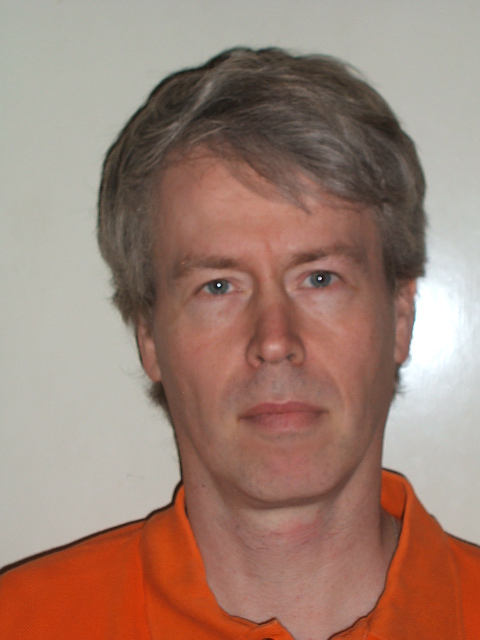
\includegraphics[height=3.5cm]{idbild.jpg}
  \textbf{Utvecklingstekniker}
  \begin{description}[nosep]
    \raggedleft\setlength\itemsep{0.1ex}\small%
  \item Objektorienterad programmering
  \item Människa-Maskin:interaktion
  \item UML
  \item C/C++
  \item Pascal
  \item Ada
  \item Python
  \end{description}
  \vspace{0.5cm}
  \textbf{Linux}
  \begin{description}[nosep,font=\sffamily\bfseries]
    \raggedleft\setlength\itemsep{0.1ex}\small%
  \item CFEngine (2012--)
  \item LINUX (RedHat 5 1997--)
  \item LINUX (Debian 2008--)
  \item Solaris (SunOS4/SunOS5)
  \item PostgreSQL
  \item Datornätverk
  \item VMWare ESXi/vSphere (använt i olika programmeringskurser)
  \item NexentaStor (använt som ett SAN/NAS, distribution via iSCSI av VMDK till ett ESXi-system bland annat)
  \end{description}
  \vspace{0.5cm}
  \textbf{Språk}
  \begin{description}[nosep,itemsep=0.1ex]
    \raggedleft\small%
  \item Svenska (modersmål)
  \item Engelska (van, samtal och skriftlig)
  \end{description}
\end{minipage}

\begin{minipage}[t]{0.73\textwidth}
  \begin{descriptioncv}{Arbeten}
    \cvitem{Servicetekniker, Kronbergs hushållsservice, Skövde}{Mars 1996--November 2006}{reparation av
      vitvaror (spisar,tvättmaskiner och småapparater) och frånluftsvärmepumpar.
      Kundkontakt med planering av arbeten. Försäljning av ersättningsmaskiner. Justering
      av ventilationssystem.}
    \cvitem{Telefonist, F6 Karlsborg}{1989-1990}{Miltex, flygvapnets radiosystem för kommunikation på flygbaser}
  \end{descriptioncv}

  \begin{descriptioncv}{Egna programmeringsprojekt}
    \cvitem{PKI:funktionalitet}{2014--}{Användning av publika certifikat med en struktur med fyra st
      certifikatutfärdare där de olika utfärdarna har olika ansvar. Rot-utfärdarens certifikat
      installeras på de system där det är nödvändigt medans mellannivåns eget certifikat
      är signerat av rotditon. Mellannivån är en delegerad rotutfärdare men med kortare löptider
      för dess eget certifikat innan rots signering av en ny utgåva. Applikations- och slutanvändare-certifikat
      hanteras av var sin specialiserad utfärdare, vars certifikat är signerad av mellannivån. Paketet är skrivet för
      openssl och dess ''ca'':verktyg.
      Eventuellt skulle man låta en utfärdaremodul lagra uppgifter om signerade certifikat i
      en CFengine datastruktur (container) för att i slutet av körningen lagra dem i en JSON:strukturerade fil för att vid
      nästa evaluering ladda in nuvarande uppgifter igen. Ett registerprogram skrivet i CFEngine:s språk }

    \cvitem{Automatisering av BIND}{2015--}{Automatiserad konfiguration av ISC:s BIND9:demon.
      Använder existerande JSON:beskrivningar av
      de olika systemen med namn, IP:adresser och vilka tjänster de har för att automatiskt generera DNS:zonbeskrivningar
      med kravet att löpnummer för zonen uppdateras på ett korrekt sätt.)}

    \cvitem{Automatisering av brandväggsregler}{2015--}{Automatiserad konfiguration av IPtable. Uppgifter om olika tjänster
      i nätet i JSON för att ange vilka avsändaradresser som är godkända för olika TCP:/UDP:portar. Acceptansför att
      kontrollera det genererade IPtable-skriptet exv inte blockerar SSH från egna maskiner. Gått igenom
      reglerna för ICMP för att ange och dokumentera varför viss trafik är nödvändig och OK eller om den är önskvärd.
      Samma typ av genomgång har gjorts för IPv6:trafik. Har via Hurricane Electric haft en globalt nåbar IPv6-adress
      i fem år jämfört med IP-onlys använding av Carrier-grade NAT.}

    \cvitem{IBM:s zXplore:program}{2021--}{har gått in i IBM:s program (tidigare känt som
      Master the Mainframe),
      för att lära mig den miljön (z/OS,COBOL,JCL,ZOWE,USS.) Ett resultat av mitt intresse för 1978:s års MVS}
  \end{descriptioncv}
\end{minipage}
\begin{minipage}[t]{0.24\textwidth}
  \raggedleft%
  \vspace{-\topskip+1cm}
  \includegraphics[height=3.5cm]{tjänstebild_Anten.jpg}
  \textbf{Andra IT:kunskaper}
  \begin{description}[nosep,itemsep=0.1ex]
    \raggedleft\setlength\itemsep{0.1ex}\small%
  \item MS Word
  \item NetBSD
  \item MVS
  \item \LaTeX
  \end{description}

  \vspace{13cm}
  \textbf{Colophon}
  \begin{description}[nosep,itemsep=0.1ex]
    \setlength\itemsep{0.1ex}\small%
  \item Stefan Skoglund {\cinzel{2021}}
  \item Gillius
  \item Cinzel (årtal)
  \item \LaTeX%
  \end{description}%
\end{minipage}%

\end{document}
